\section{Evaluation \& agreement}
\subsection{Requirements evaluation}
Ci sono alcuni aspetti che definiscono in modo concerto come valutare i requisiti in maniera rigorosa. Vediamo i punti caratterizzanti della fase di valutazione degli requisisti:
\begin{itemize}
  \item \textit{inconsistency management}, quindi identificazione e risoluzione delle inconsistenze. Questi potrebbero corrispondere, ad esempio, alla gestione conflittuale di due punti di vista differenti da parte di due stakeholders al fine di trovare un accordo. Quello che comprende sono:
  \begin{itemize}
    \item tipi di inconsistenza
    \item gestione delle stesse 
    \item gestione dei conflitti in modo sistematico
  \end{itemize}
  \item la valutazione di alternative per prendere decisioni, una tecnica da adottare potrebbe prevedere la selezione dell'alternativa "preferita".
  \item la prioritizzazione dei requisti, \textit{requirements prioritization}; usata per risolvere conflitti, porre vincoli per costi/tempistiche. Fase che inoltre è intenta a supportare lo sviluppo incrementale.
\end{itemize}

\subsubsection{Inconsistency management}
Definiamo \textbf{inconsistenza} come la violazione della regola di coerenza tra gli elementi, le inconsistenze sono molto frequenti nell'ambito del requirments engineering e si ha una distinzione dei tipi di incosistenza: 
\begin{itemize}
    \item \textbf{inter‐viewpoints}, quando ogni stakeholder ha il suo obiettivo primario e diverse preoccupazioni a riguardo, ad esempio uno stakeholder del dipartimento di marketing avrà obiettivi e altre valutazioni da effettuare rispetto ad un esperto del dominio applicativo.
    \item \textbf{intra‐viewpoints}, quando si hanno conflitti tra i requisti di qualità (qualitativi) (conflitti per esempio tra sicurezza e accessibilità)
\end{itemize}
Le in devono identificate e risolte, dal punto di vista dei tempi:
\begin{itemize}
  \item \textit{non troppo presto}, per avere prima un'elicitation più approfondita 
  \item \textit{non troppo tardi}, per permettere lo sviluppo del software, questo perché ci si potrebbe ritrovare con un prodotto dove qualsiasi cosa può essere stata sviluppata da specifiche incoerenti.
\end{itemize}

Possiamo distinguere diverse tipologie di inconsistenza:
\begin{itemize}
  \item \textbf{terminology clash}, avendo lo stesso concetto denominato diversamente in statement diversi. 
  \item \textbf{designation clash}, avendo lo stesso nome per concetti diversi in statement diversi
  \item \textbf{structure clash}, avendo lo stesso stesso strutturato in modo diverso in statement diversi
\end{itemize}

Distinguiamo inoltre:
\begin{itemize}
  \item \textbf{conflitto forte}, avendo statement non soddisfacibili contemporaneamente (ad esempio $S\land \neg S$)
  \item \textbf{conflitto debole (\textit{divergenza})}, avendo statement non soddisfacibili contemporaneamente in certe condizioni e con certi vincoli
\end{itemize}

Per gestire i clash (scontri) in termini di terminologia, designazione dei compiti e struttura si usa il glossario costruito nella fase di elicitation (dove vengono anche usati eventualmente acronimi).\\
In entrambe le due classi, debole e forte, dei conflitti più sono difficili da gestire, più profonde(grandi) sono le cause (danni) generate, identifichiamo come cause:
\begin{itemize}
  \item obiettivi personali in conflitto da parte degli stakeholder. Questa cosa che andrebbe gestita alla base propagandone i risultati al livello dei requirements
  \item legati ad alcune preoccupazioni di natura non funzionale, come ad esempio prestazioni vs sicurezza. Questa cosa che andrebbe gestita tramite uno studio dei tradeoff, i compromessi, migliori
\end{itemize}

\subsection{Gestione dei conflitti}

Come detto la gestione dei conflitti avviene in modo sistematico seguendo i punti denominati nel schema:
\begin{figure}[H]
    \centering
    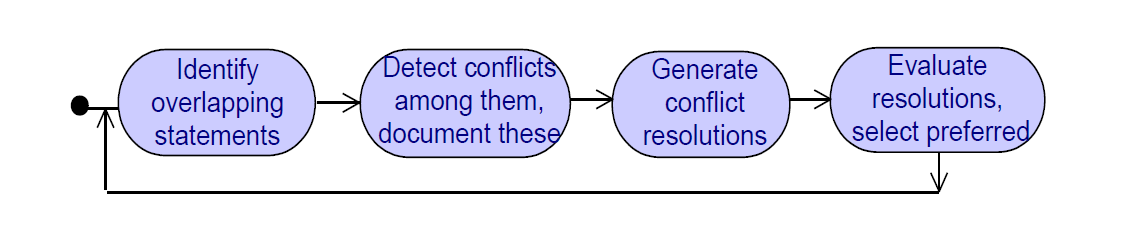
\includegraphics[scale = 0.5]{Imm/manage_conflicts.PNG}
\end{figure}
\begin{itemize}
    \item Identificare di sovrapposizione degli statements, fa riferimento a termini o fenomeni comuni. Si potrebbero assumere delle precondizioni per dichiarazioni contrastanti.
    \item La seconda fase corrispondente al rilevamento dei conflitti, può essere fatto informalmente, tramite euristiche sulle categorie dei requisiti in conflitto, o formalmente. \\
    Conflitti rilevati dovrebbero essere documentati per una successiva risoluzione e analisi dell'impatto. Si usano strumenti come l'\textbf{interaction matrix} che presenta su righe e colonne gli statement e negli incroci indica: 
    \begin{itemize} 
        \item 1 per il conflitto 
        \item 0 per nessun overlap 
        \item 1000 per overlap senza conflitto 
    \end{itemize} 
    Avendo, per ogni statement $S_i$, indicando con $S_i$ la riga/colonna corrispondente (sono uguali):\\
    $conflict(S_i)= \displaystyle \left(\sum_{s\in S_i}s\right) \mod 1000\quad$ e 
    $\quad nonConflictingOverlaps(S_i)=  \displaystyle \Bigl\lfloor{ \left(\sum_{s\in S_i}s \right) } \// {1000}\Bigr\rfloor$
    \item La terza fase, quando generiamo una soluzione ai conflitti riscontrati, per migliori risultati sarebbe meeglio:
        \begin{itemize}
            \item considerare e valutare \textbf{PRIMA} più soluzioni possibili, queste solo le soluzioni candidate ad essere le migliori
            \item confrontare, selezionare (o concordare) quale sia la migliore/la preferita \textbf{DOPO}
        \end{itemize}
    Teniamo ben presente che la generazione delle soluzioni candidate vengono generate tramite tecniche di elicitation e usando tattiche di risoluzione dei conflitti, quali:
        \begin{itemize}
          \item evitare condizioni con limite imposto 
          \item ripristinare statement in conflitto
          \item indebolire gli statement in conflitto
          \item non considerare statement a bassa priorità
          \item approfondire source e target del conflitto
        \end{itemize}
     \item Quarta fase prevede l'uso di vari criteri per la scelta della soluzione migliore/preferita, questi criteri sono:
        \begin{itemize}
            \item contributo a requisiti non funzionali critici 
            \item contributo alla risoluzione di altri conflitti e rischi 
            \item applicazione dei principi di \textit{risk analysis}
        \end{itemize}
\end{itemize}
\subsection{Requirements Prioritization}
Ai vari requisti (elictred e valutati) va imposta una prioritizzazione in termini di:
\begin{itemize}
  \item risoluzione dei conflitti 
  \item limitazioni delle risorse (budget, personale, programmi) 
  \item sviluppo incrementale 
  \item ripianificazione a causa di problemi imprevisti
\end{itemize}
Alcuni principi che vengono utilizzati per una prioritizzazione efficiente sono:
\begin{enumerate}
  \item ottenere pochi livelli ordinati di uguale priorità
  \item utilizzare livelli relativi ("maggiore di" etc$\ldots$) 
  \item avere requisiti comparabili: stessa granularità, stesso livello di astrazione 
  \item utilizzare requisiti non mutuamente dipendenti (uno può essere mantenuto, un altro eliminato) 
  \item tramite un'accordo con i vari partecipanti e stakeholder
\end{enumerate}
Per i primi tre posso usare una tecnica sistematica basata su diversi step:
\begin{itemize}
  \item stimare il contributo relativo di ogni richiesta al \textbf{valore} del progetto 
  \item stimare il contributo relativo di ciascuna richiesta al \textbf{costo} del progetto 
  \item tracciare il \textbf{diagramma valore-costo}
\end{itemize}
\begin{figure}[H]
    \centering
    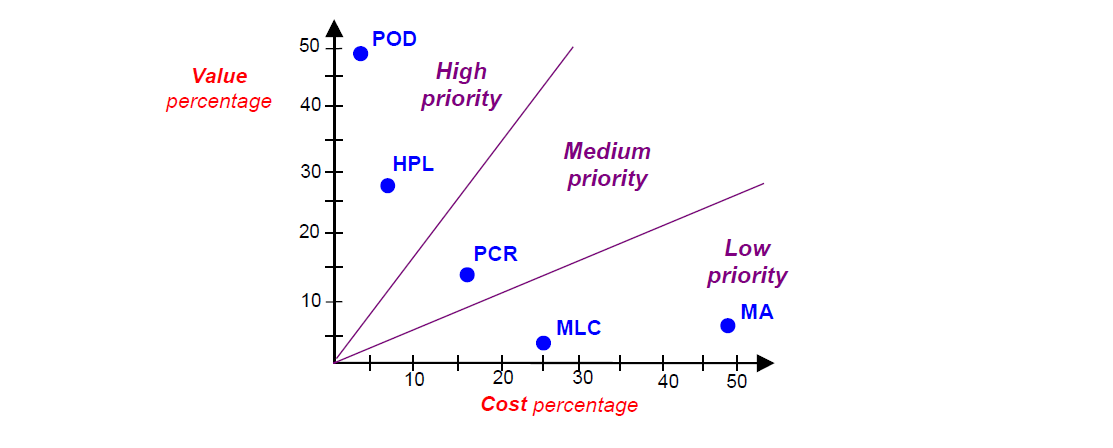
\includegraphics[scale = 0.5]{Imm/plot.PNG}
\end{figure}

Si usa quindi la tecnica AHP dalla \textbf{Decision Theory} dove si cerca di determinare in che proporzione ogni requisito $R_i$, con $i = 1, \dots, N$, contribuisce al criterio $Crit$. Il crietrio $Crit$ viene applicato due volte; la prima volta in funzione del \textbf{Valore}, $Crit=value$, e poi per il \textbf{costo}, $Crit=cost$.\\
Si hanno quindi due step:
\begin{enumerate}
  \item Costruire la \textbf{comparison matrix}, questo ci aiuta a stimare quanto il i-esimo requisito $R_i$, contribuisce al criterio, quando messo a confronto con il j-esimo requisito $R_j$
  \item Determinare come il criterio $Crit$ si distribuisce all'interno di tutti i requisiti $R_i$
\end{enumerate} 

Avevamo detto di utilizzare \textbf{AHP} per il confronto. Questa tecnica esegue 2 step, che prima vengono eseguiti con criterio "Value" e alla seconda iterazione con criterio "cost":
\begin{enumerate}
    \item Confronta i requisiti a coppie. Per poterlo fare inizialmente si usa matrice. Ogni elemento $R_{ij}$ della matrice rappresenta l'importanza del i-esimo criterio relativo al j-esimo criterio. Se il valore $R_{ij}$ è maggiore di 1, ci indica che i-esimo criterio è più importante del j-esimo. L'importanza viene concordata su una scala da 1 a 9. Quindi se il valore di $R_{ij}$ è: 
        \begin{itemize}
            \item 1, allora $i$ e $j$ sono equamente importanti
            \item 3, allora $i$ è poco più importante di $j$
            \item 5, allora $i$ è più importante di $j$
            \item 7, allora $i$ è molto più importante di $j$
            \item 9, allora $i$ è definitivamente più importante di $j$
        \end{itemize}
        All'interno della matrice i valori di $R_{ji} =\displaystyle \frac{1}{R_{ij}}$
    \item Nella seconda parte viene valutato come il criterio si distribuisce all'interno di tutti i requisiti. Si costruisce quindi la matrice che ci permette di effettuare sempre un confronto a coppie, ma con valori normalizzati. Normalizzati perché la somma delle colonne corrisponde a $1$. Ogni colonna è calcolate come: $$\overline{R_{ij}} = \displaystyle\frac{R_{ij}}{\sum_i(R_{ij})}$$ Il contributo del requirment è quindi poi dato eseguendo la media sulle righe:
    $$Contrib(R_j, Crit) = \frac{\sum_i(\overline{R_{ij}})}{N}$$
\end{enumerate}